\subsection{Prime-Time Ratio} \label{subsec:primetime}

The daily diurnal nature of usage patterns across many
households naturally requires the provider to design networks capable of handling 
load at the peak times in a day. Such peak times are usually observed during
evening hours, and the data transferred at this time is called peak usage.
The FCC defines \textbf{Prime Time} as the local time from 7:00 PM to 11:00
PM~\cite{fcc2014measuring-broadband}, when many
households heavily consume real-time entertainment traffic (video), seen as primarily
responsible for high usage during these hours. Latency and performance are adversely
affected during prime-time, causing bottlenecks at home, the last mile, in
transit, or at the content server. For example, the Sandvine Global
Internet Phenomena Report \footnote{The Sandvine Reports ~\cite{sandvine20141h,
sandvine20142h}are released bi-annually and
contain a detailed analysis of aggregate Internet usage. They are also referred
to in the FCC reports~\cite{fcc2015progress-report, fcc2014measuring-broadband,
fcc2014progress-report}} showed that devices in the same household selected Netflix's
own CDN (OpenConnect) during off-peak hours, and third party CDNs (with differing
performance) during prime-time. This may happen because Netflix OpenConnect is over-utilized
during prime time~\cite{sandvine20141h}.

To measure the concentration of network usage during prime time,
Sandvine defined the \textbf{Prime-Time ratio} as the ``absolute levels of network traffic
during an average peak period hour with an average off-peak hour''. Based on the FCC
definition of prime-time hours (7p-11p), we measure the daily prime-time ratio of the \control{} group and compare it to the \treatment{}. Prime-time ratio is definded by dividing the the average traffic data rate during an average prime-time hour, by the off-peak average traffic rate.

Prompted by the monotonically increasing trend of usage behavior during daytime hours on
weekdays (figure~\ref{fig:TS-data-rate-daily})
we calculated the prime-time ratio for each four hour period throughout the day
to find the evening hours with the largest ratio.
In our dataset, the prime time ratio peaks at 8:00 PM -- 12:00 AM,
rather than FCC's definition of 7:00 PM -- 11:00 PM. This discrepancy could be limited
only to the high tier households in our dataset, but we deem that unlikely.
%as the demand for traffic during prime time should be independent of the tier.
Another reason could be that prime time is delayed globally with the rise in real
time entertainment's contribution to traffic.

\begin{figure}[ht]
\begin{minipage}{\linewidth}
\centering
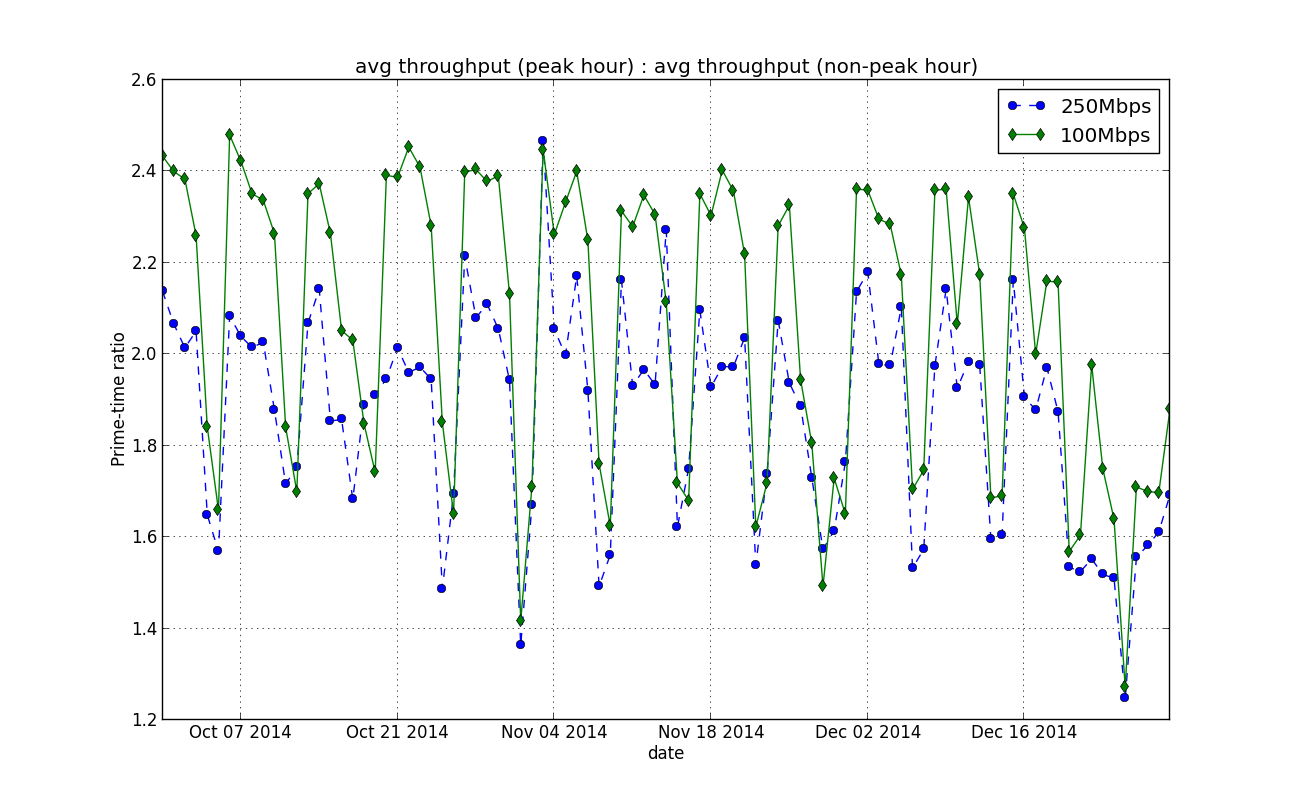
\includegraphics[width=\linewidth]{figures/prime-time-ratio-by-date[replace].png}
\caption{Prime Time ratio showing weekly pattern + differences during holiday periods (Thanksgiving, Christmas)}
%http://riverside.noise.gatech.edu:8083/separated/full/prime-time-ratio-by-date.png
\label{fig:TS-prime-time-ratio}
\end{minipage}
\end{figure}

We use our updated definition of Prime Time (table~\ref{tab:eval-criteria}) to calculate and plot
the Prime Time ratio per day for the \treatment{} and \control{} groups in
figure~\ref{fig:TS-prime-time-ratio}. A comparison shows that
the \treatment{} set's prime time ratio is unexpectedly 10\% lower than the \control{} group. This supports our initial observation [\autoref{subsec:behavior}] that showed that the usage during peak evening hours is similar
across both groups, but the usage in off peak hours is higher in the \treatment{}.